\documentclass[12pt,a4paper]{article}

% ===== LuaLaTeX: современные векторные шрифты =====
\usepackage{fontspec}           % для работы с TrueType/OpenType шрифтами
\setmainfont{Times New Roman}   % или Arial, Libertinus Serif, etc.

% ===== Языки и кодировка =====
\usepackage[english,russian]{babel}
\usepackage{csquotes}           % для кавычек

% ===== Математика =====
\usepackage{amsmath}
\usepackage{amsfonts}
\usepackage{amssymb}

% ===== Графика =====
\usepackage{graphicx}
\usepackage{tikz}
\usepackage{tkz-euclide}
\usepackage{pgfplots}
\pgfplotsset{compat=1.18} 

\usetikzlibrary{patterns}
\usepackage{float}
\usepackage{wrapfig}

% ===== Таблицы =====
\usepackage{multirow}
\usepackage{booktabs}
\usepackage{siunitx}
\usepackage{array}

% ===== Оформление =====
\usepackage[left=1cm,right=1cm,top=1cm,bottom=2cm]{geometry}
\usepackage{setspace}
\usepackage{indentfirst}
\usepackage{microtype}          % улучшает качество шрифтов
\usepackage{hyperref}

% ===== Вспомогательное =====
\usepackage{calc}
\usepackage{subfigure}

\usepackage{listings}
\usepackage{xcolor}

% Настройки для Python
\lstset{
	language=Python,
	basicstyle=\ttfamily\small,
	keywordstyle=\color{blue}\bfseries,
	stringstyle=\color{red},
	commentstyle=\color{green!50!black},
	numbers=left,
	numberstyle=\tiny\color{gray},
	stepnumber=1,
	numbersep=5pt,
	backgroundcolor=\color{gray!10},
	frame=single,
	breaklines=true,
	breakatwhitespace=true,
	tabsize=4,
	showspaces=false,
	showstringspaces=false,
	captionpos=b
}

\title{Изучение аттракторов с помощью численных методов}
\author{Тодоров Николай}
\date{\today}

\begin{document}
	\maketitle
Изучим систему нелинейных дифференциальных уравнений первого порядка

\begin{equation}
	\begin{cases}
		\dot{x} = \sigma (y - x) \\
		\dot{y} = x(r-z) - y \\
		\dot{z} = xy - bz
	\end{cases}
\end{equation}

Эта система называется системой Лоренца. Эту систему Эдвард Лоренц получил, когда изучал конвекцию в атмосфере Земли. Для нахождения ее численного решения мы воспользуемся методом Рунге-Кутта 4-го порядка

\[
\begin{array}{c|cccc}
	0 & 0 & 0 & 0 & 0\\
	1/2 & 1/2 & 0 & 0 \\
	1/2 & 0 & 1/2 & 0 & 0 \\
	1 & 0 & 0 & 1 & 0 \\
	\hline
	& 1/6 & 2/6 & 1/6 & 1/6
\end{array}
\]

\begin{lstlisting}
	def solve(sigma, r, b, x0, y0, z0, number, T):
	    t = np.linspace(0, T, number)
	    h = t[1] - t[0]
	    sol = np.zeros((3, number))
	    sol[0, 0] = x0
	    sol[1, 0] = y0
	    sol[2, 0] = z0
	    for i in range(0, number - 1):
	        xi, yi, zi = sol[:, i]
	        k_1 = f(sigma, r, b, xi, yi, zi)
	        k_2 = f(sigma, r, b, xi + h * k_1[0]/2, yi + h * k_1[1]/2, zi + h * k_1[2]/2)
	        k_3 = f(sigma, r, b, xi + h * k_2[0]/2, yi + h * k_2[1]/2, zi + h * k_2[2]/2)
	        k_4 = f(sigma, r, b, xi + h * k_3[0], yi + h * k_3[1], zi + h * k_3[2])
	        sol[:, i + 1] = sol[:, i] + h * (k_1 + 2 * k_2 + 2 * k_3 + k_4)/6
	    x = sol[0, :]
	    y = sol[1, :]
	    z = sol[2, :]
	
	    return t, x, y, z
\end{lstlisting}

У этого метода погрешность порядка $O(h^5)$ на каждом шаге и $O(h^4)$ суммарно на отрезке. Он является стандартом для изучения хаоса, так как сочетает высокую точность и относительно простую реализацию.

Эта система при $r \ge 1$ имеет три точки равновесия:

\[A = (0, 0, 0)\]
\[B = (\sqrt{b(r-1)},\sqrt{b(r-1)}, r-1) \text{, }\]
\[C = (-\sqrt{b(r-1)}, -\sqrt{b(r-1)}, r-1)\]

Нам будет интересовать решение при следующих значениях параметров:

\[\sigma = 10 \text{, } r = 28 \text{, } b = 8/3\]

Рассмотри два решения с разными начальными условиями, отличающимися на малую величину (порядка $10^{-5}$). Построим фазовый портрет обоих решений в 3D-пространстве, рядом отобразим зависимость расстояния (в смысле евклидовой нормы) между двумя решениями от времени. Как мы можем видеть, сначала точки движутся абсолютно одинаково, затем в какой-то момент времени они расходятся и живут отдельно друг от друга. Малая ошибка вначале экспоненциально возрастает. Это пример так называемого странного аттрактора. Формальное определение аттрактора следующее: это подмножество в фазовом пространстве, к которому стремятся фазовые кривые системы в течение продолжительного времени. Слово «странный» в данном контексте значит, что аттрактор имеет сложную, фрактальную структуру; траектории такого аттрактора не замыкаются, а малые отклонения очень быстро накапливаются (по экспоненциальному закону).

Это означает, что, \textbf{даже используя мощный компьютер, мы не можем просчитать траекторию, проходящую вблизи аттрактора, с разумной точностью на протяжении длительного промежутка времени. На каждом шаге вычислений неизбежно вносятся ошибки (из-за округления чисел и погрешностей численных методов), которые быстро накапливаются и приводят к тому, что найденная траектория сильно отличается от настоящей}.

Такое искажение невозможно исправить, просто увеличивая мощность компьютера. Подобное явление называется «динамическим хаосом».

\begin{figure}[H]
	\centering
	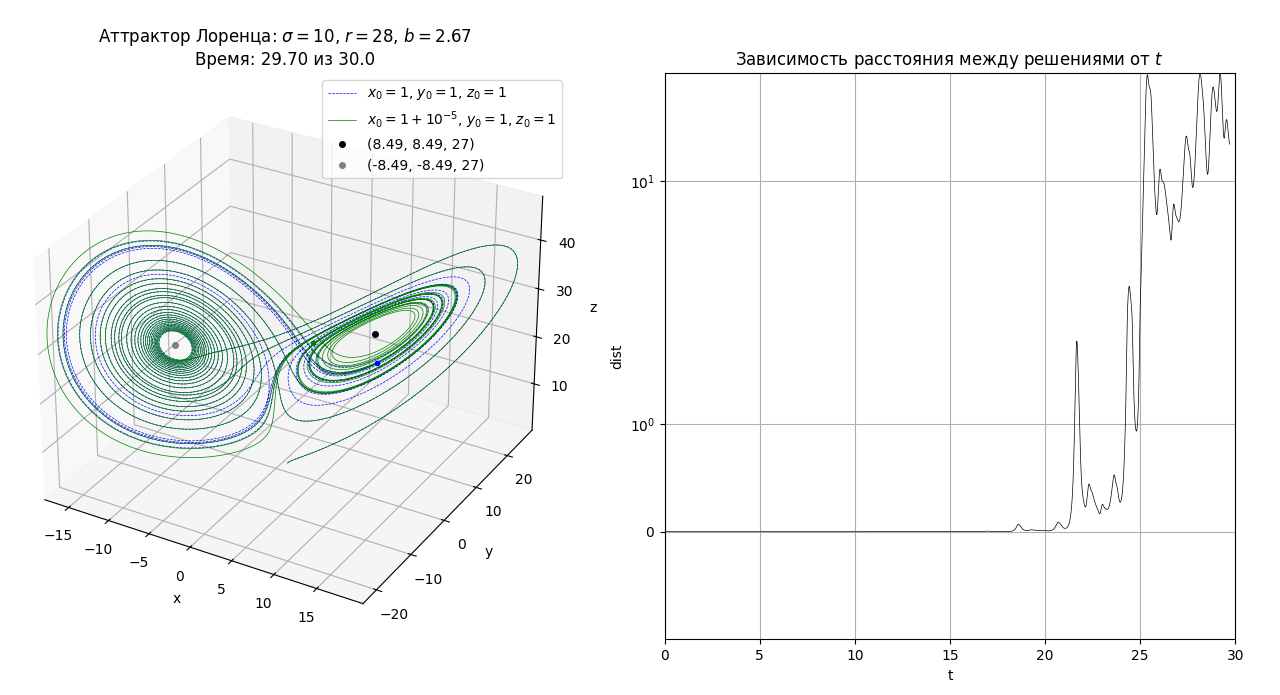
\includegraphics[width=1\textwidth]{Аттрактор_Лоренца}
	\caption{Аттрактор Лоренца}
\end{figure}

\begin{figure}[H]
	\centering
	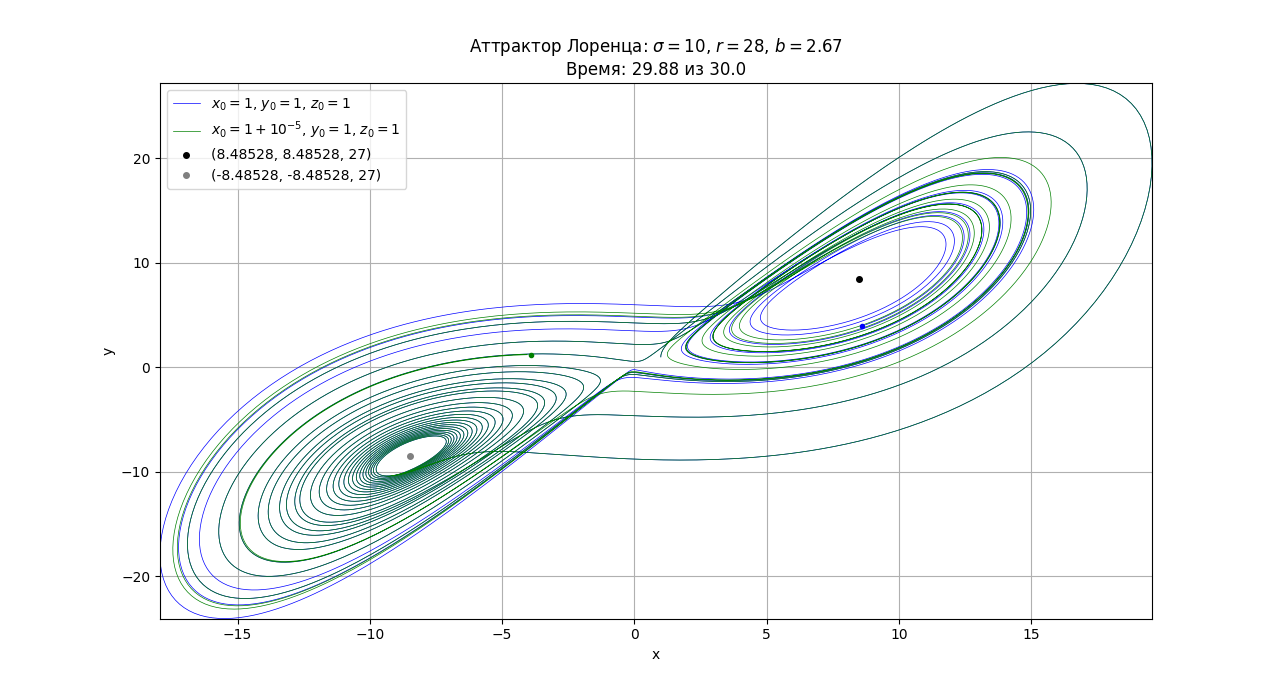
\includegraphics[width=1\textwidth]{Аттрактор_Лоренца_2D}
	\caption{Аттрактор Лоренца в XY}
\end{figure}

Аттрактор внешне похож на бабочку; каждое из ее крыльев имеет фокус $B$ и $C$ соответственно.

Покажем как выглядят графики зависимостей координат от времени. Выполним также преобразование Фурье от них (используя FFT с помощью библиотечной функции в numpy) и посмотрим на спектр частот (он будет достаточно широкий)

\begin{figure}[H]
	\centering
	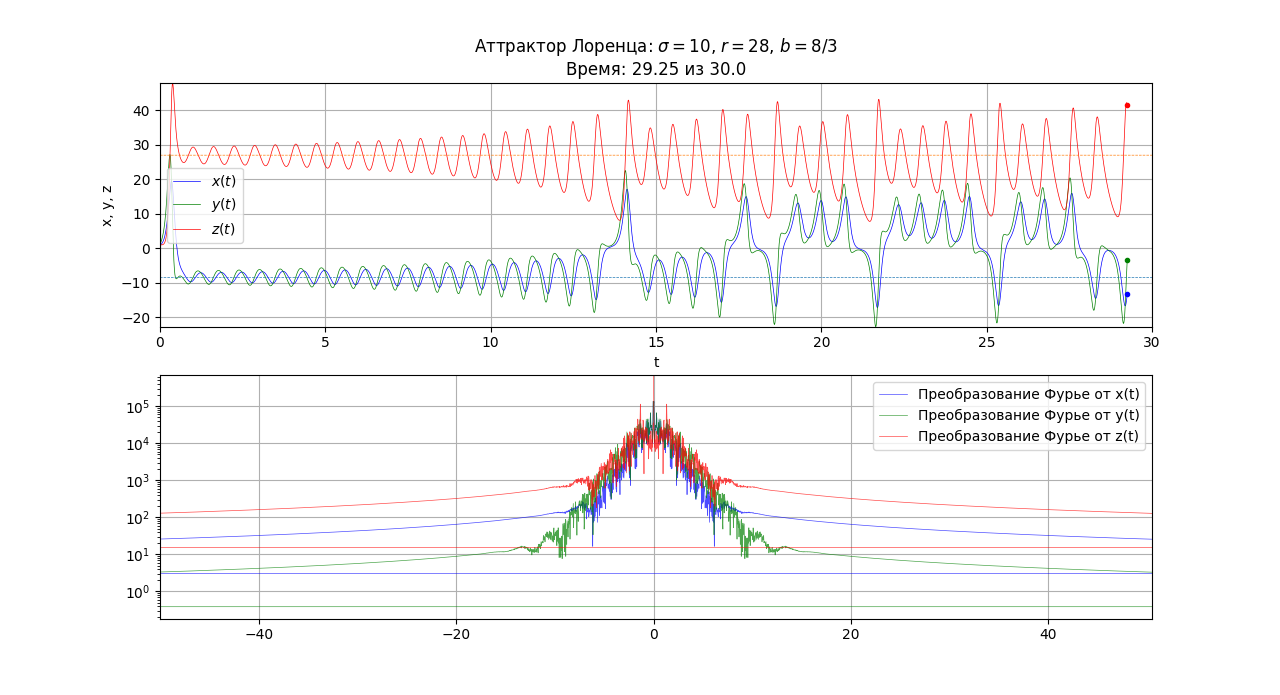
\includegraphics[width=1\textwidth]{Аттрактор_Лоренца_1}
	\caption{Временные зависимости координат аттрактора Лоренца и их фурье-спектры}
\end{figure}

Теперь посмотрим, как выглядит бифуркационная диаграмма данной системы. В качестве регулирующего параметра мы возьмем $r$, который будет изменяться от 0.01 до 30. По вертикальной оси мы будем откладывать локальные максимумы координаты $x$. Процесс нахождения этих максимумов описывается ниже написанным кодом

\begin{lstlisting}
	for r in r_vals:
	    t, x, y, z = solve(sigma, r, b, x_0, y_0, z_0, number, T)
	    x = x[2500:]
	    x_r_max = []
	    for i in range(1, len(x) - 1):
	        if x[i - 1] < x[i] > x[i + 1]:
	        x_r_max.append(x[i])
	        x_max.append(x_r_max)
\end{lstlisting}

Разбить полученную диаграмму можно на три участка: на первом - максимумы расположены выше нуля, на втором - нижу нуля, на третьем - как выше нуля, так и ниже нуля. Концептуально это означает следующее: при малых значениях параметра $r$ фазовые кривые притягиваются к точке равновесия $B$, при средних - к точке $C$; при достаточно больших значениях этого параметра решение не стремится к какому-либо фокусу, оно периодически сменяет крыло и не затухает в отличие от решений при малых $r$.

\begin{figure}[H]
	\centering
	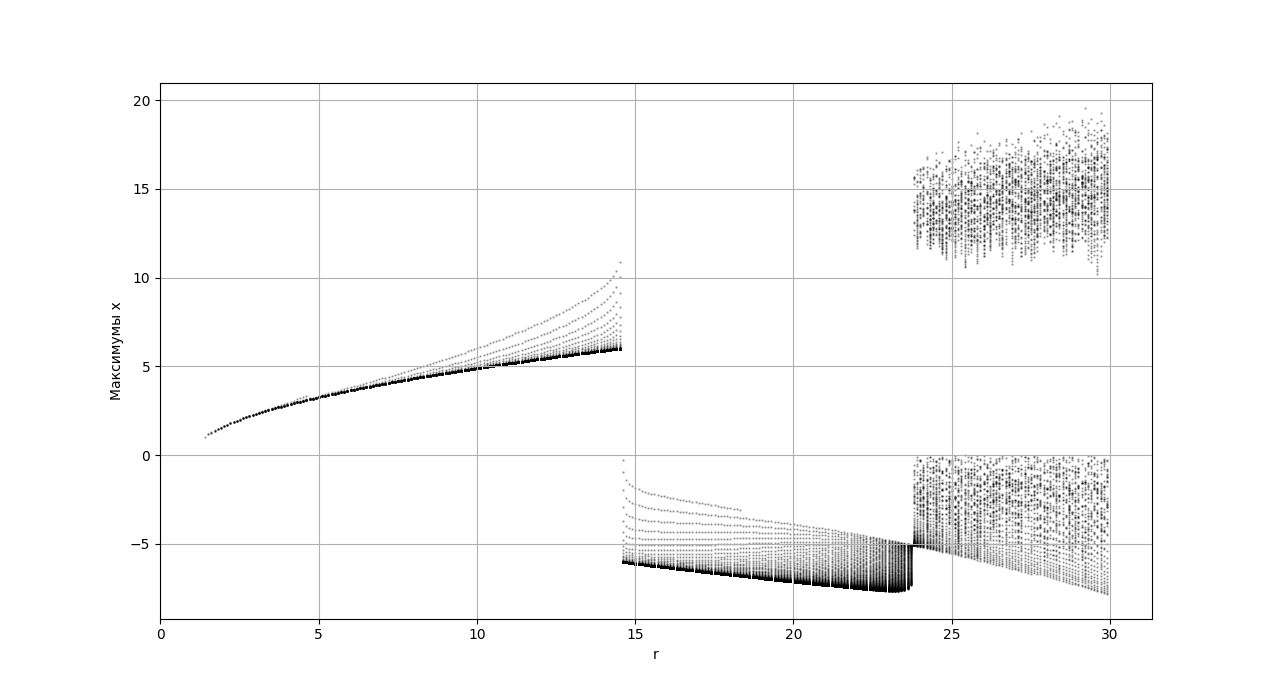
\includegraphics[width=1\textwidth]{Бифуркационная_диаграмма}
	\caption{Бифуркационная диаграмма}
\end{figure}
\end{document}